% Preamble
\documentclass[../Relazione_circuiti]{subfiles}

% Packages

\graphicspath{{\subfix{../images/}}}

% Document
\begin{document}

\subsection{Analisi preliminare qualitativa}

  \begin{figure}[H]
    \centering

    \begin{subfigure}[b]{0.3\textwidth}
      \centering
      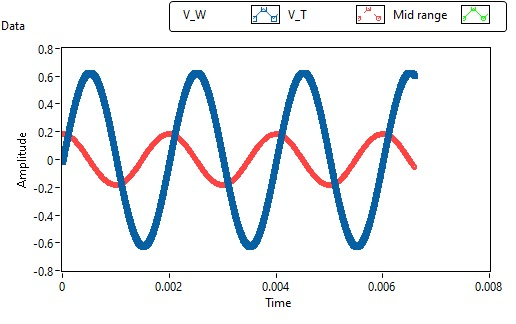
\includegraphics[width=\textwidth]{Cross_waveform_500.jpeg}

      \caption{Segnali a 500Hz}
      \label{fig:signal_500}

    \end{subfigure}
    \begin{subfigure}[b]{0.3\textwidth}
      \centering
      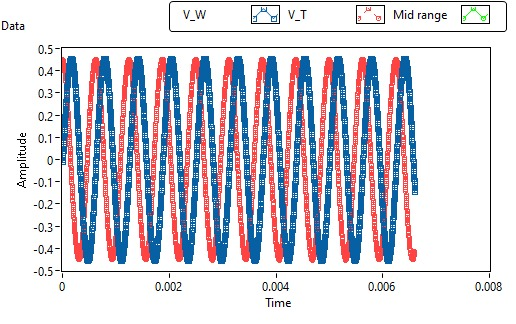
\includegraphics[width=\textwidth]{Cross_waveform_1600.jpeg}

      \caption{Segnali a 1600Hz}
      \label{fig:signal_1600}

    \end{subfigure}
    \begin{subfigure}[b]{0.3\textwidth}
      \centering
      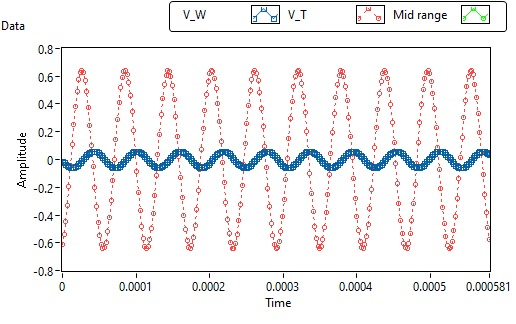
\includegraphics[width=\textwidth]{Cross_waveform_17000.jpeg}

      \caption{Segnali a 17kHz}
      \label{fig:signal_17k}

    \end{subfigure}
    \hfill

    \caption{Segnali osservati sui rami Woofer (blu) e Tweeter (rosso)
      a frequenza fissata.}
    \label{fig:signal_waveforms}

  \end{figure}

  La figura \ref{fig:signal_waveforms}
  mostra la forma d'onda dei segnali osservati sui rami Woofer e Tweeter in risposta ad un segnale sinusoidale. La
  figura \ref{fig:signal_1600} mostra il comportamento nei pressi della frequenza di cross attesa, la figura
  \ref{fig:signal_500} a 1/3 e la figura \ref{fig:signal_17k} a circa 10 volte.

  Si osserva (Figura \ref{fig:signal_1600}
  ) che, coerentemente con quanto atteso, i segnali hanno ampiezza simile nei pressi di $f_{cross}$
  . A basse frequenze si osserva (Figura \ref{fig:signal_500}) un'attenuazione del 60\%
  dell'ampiezza sul ramo Tweeter e nessuna alterazione sul Woofer, ad alte frequenze un'attenuazione sul Woofer
  dell'86\% e nessuna sul Tweeter (Figura \ref{fig:signal_17k}).

\subsection{Analisi della frequenza misurata}

\subsection{Analisi dell'ampiezza}

\begin{figure}[H]
\centering

\begin{subfigure}{=0.7\textwidth}

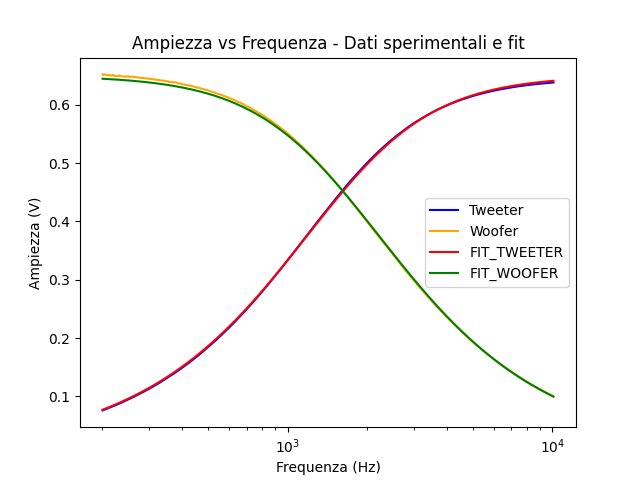
\includegraphics[width=\textwidth]{cross.png}

\end{subfigure}

\caption{Ampiezza misurata in funzione della frequenza (asse della frequenza in scala logaritmica). A causa della scala le incertezze sulle singole misure non sono visibili. L'andamento è rappresentato da una linea continua a causa dell'alta densità di punti.}
\label{fig: cross_amplitude}

\end{figure}

La figura \ref{fig: cross_amplitude} mostra l'andamento di ampiezza dei segnali filtrati in funzione della frequenza. 

La relazione funzionale Ampiezza massima-Frequenza (misurata ai capi della resistenza di carico dei rami) è data da:

\begin{equation}
V_{woofer} = \frac{V_{in}}{\sqrt{R^2+(\omega L)^2}}
\end{equation}

\begin{equation}
V_{tweeter} = \frac{V_{in}}{\sqrt{R^2+(\frac{1}{\omega C})^2}}
\end{equation}

dove $V_{in}$ rappresenta la tensione in ingresso (assunta costante) pari a 0.65, osservata nel ramo Woofer nel limite di basse frequenze e nel ramo Tweeter nel limite di alte frequenze.

E' stato effettuato un fit ai parametri L e C (R assunta costante). Da essi è stata poi ricavata la frequenza di crossover secondo l'Eq. \ref{eq:f_cross}. 

\begin{tabular}{c | c }

%Heading
Grandezza & Valore \\

L & $(10.13 \pm 0.01)$ mH \\
C & $(953.39 \pm 0.05)$ nF

\end{tabular}

\subsection{Analisi della fase}

\begin{figure}[H]
\centering

\begin{subfigure}{=0.5\textwidth}
\centering
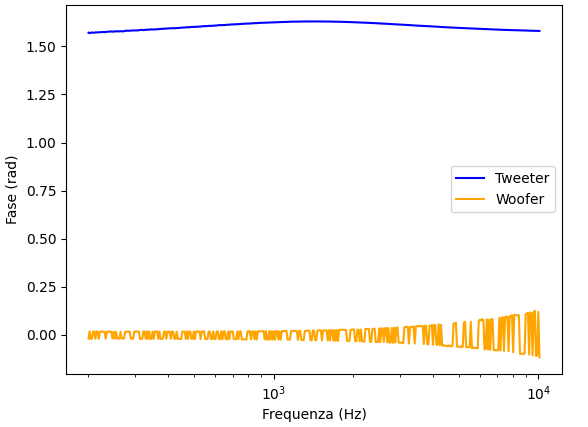
\includegraphics[width=12cm]{phase_dataonly.png}

\caption{Sfasamento Tweeter-Woofer (solo dati)}
\label{fig: pdiff_dataonly}

\end{subfigure}

\begin{subfigure}{=0.5\textwidth}
\centering
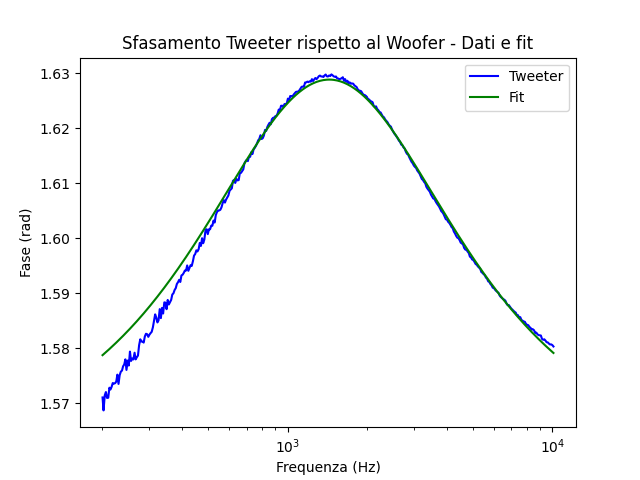
\includegraphics[width=12cm]{phase_cross.png}

\caption{Dati e sovrapposizione con fit}
\label{fig: pdiff_fit_data}

\end{subfigure}

\caption{Fase del Tweeter misurata rispetto al Woofer (blu). Fase del Woofer  misurata rispetto se stesso (giallo). La frequenza è in scala logaritmica. Le incertezze non sono visibili a causa della scala.}
\label{fig: phase_diff}

\end{figure}

La figura \ref{fig: pdiff_dataonly} mostra lo sfasamento relativo Tweeter-Woofer (curva Tweeter in figura), che segue la relazione funzionale:

  \begin{equation}
    \label{eq:p_diff}
    \phi_{diff} \; = \; \arctan(\frac{\omega L}{R}) + \arctan(\frac{1}{\omega RC})
  \end{equation}
  
Tramite uno studio di funzione si può dimostrare che lo sfasamento relativo è massimo alla frequenza di cross e vale:


 \begin{equation}
    \label{eq:p_diff_cross}
    \phi_{cross} \; = \; 2 \arctan(\frac{1}{R} \sqrt{\frac{L}{C}})
  \end{equation}

  
Effettuando un fit all'Eq (\ref{eq:p_diff}), abbiamo ricavato i valori L e C, considerando invece R come parametro costante poiché la frequenza di cross non dipende da esso.


\begin{table}[H]
\centering

\begin{tabular}{c | c | c}
%Heading
Grandezza & Valore & Unità di misura \\
\hline
L & $ 11.82 \pm 0.03 $ & mH \\
C & $ 1.037 \pm 0.002 $ & $\mathrm{\mu}$F \\
$f_{cross}$ & $ 1437 \pm 2$ & Hz

\end{tabular}
\caption{Risultati del fit dell'Eq \ref{eq:p_diff}}
\label{tab: fit_phase}

\end{table}
%ribadisco per chiarezza
Ai dati è stata assegnata un'incertezza casuale stimata mediante fit alla forma d'onda osservata per ogni frequenza, come descritto in sezione 2. 

Inoltre, poiché l'acquisizione dei due canali non è simultanea ma sequenziale (mediante multiplexer che itera sui canali Analog Input) si ha che tra due canali acquisiti consecutivamente (come nel nostro caso) vi è uno sfasamento temporale tra l'inizio delle due acquisizioni, che risulta essere pari a $\tau_{aq}=1 \mu \mathrm{S}$ secondo le specifiche di ELVIS, che si riflette in un errore sistematico sulla fase, che risulta essere inferiore al valore vero.

Questo è stato corretto aggiungendo alla fase misurata  $ 2 \pi f \tau_{aq}$, dove $f$ rappresenta la frequenza del segnale (si veda l'appendice per una spiegazione approfondita).

In figura \ref{fig: phase_diff} si nota che la fase del Woofer rispetto se stesso, che ci aspettavamo essere 0 poiché il trigger è sul medesimo canale, risulta in realtà non nulla ma oscillante attorno a questo valore. L'ampiezza di dette oscillazioni aumenta all'aumentare della frequenza. Questo fenomeno è stato osservato anche sulla fase del tweeter e la cosa è coerente con il fatto che la fase del tweeter è misurata relativamente al Woofer: una fluttuazione nello 0 della fase si ripercuote su tutte le altre misure. Abbiamo corretto queste fluttuazioni sul canale Tweeter sottraendo i valori misurati sul canale Woofer. Questo non ha influenzato il valore medio di sfasamento del Tweeter ad una data frequenza poiché la fase del Woofer è in media 0.


\end{document}